\documentclass[a4paper,oneside,14pt]{extreport}

\usepackage[T2A]{fontenc}
\usepackage[utf8]{inputenc}
\usepackage[english,russian]{babel}

\usepackage[left=30mm, right=10mm, top=20mm, bottom=20mm, bindingoffset=0cm]{geometry}

\usepackage{microtype}
\usepackage{tikz}

\usepackage{setspace}
\onehalfspacing
\usepackage{graphicx}
\usepackage{indentfirst}
\setlength{\parindent}{12.5mm}

\usepackage{titlesec}
\titleformat{\chapter}{\LARGE\bfseries}{\thechapter}{10pt}{\LARGE\bfseries}
\titlespacing*{\chapter}{0pt}{-20pt}{10pt}
\titleformat{\section}{\large\bfseries}{\thesection}{10pt}{\large\bfseries}
\titlespacing*{\section}{0pt}{0pt}{10pt}
\titleformat{\subsection}{\normalsize\bfseries}{\thesubsection}{10pt}{\normalsize\bfseries}
\titlespacing*{\subsection}{0pt}{5pt}{5pt}

\addto{\caption}{\renewcommand*{\contentsname}{Содержание}}
\usepackage[square,sort,comma,numbers]{natbib}
\renewcommand{\bibsection}{\chapter*{Список литературы}}

\usepackage{caption}

\usepackage{wrapfig}
\usepackage{float}
\usepackage{listings}
\usepackage{graphicx}
\graphicspath{{.}}
\newcommand{\imgwc}[4]
{
	\begin{figure}[#1]
		\center{\includegraphics[width=#2]{inc/img/#3}}
		\caption{#4}
		\label{img:#3}
	\end{figure}
}
\newcommand{\imghc}[4]
{
	\begin{figure}[#1]
		\center{\includegraphics[height=#2]{inc/img/#3}}
		\caption{#4}
		\label{img:#3}
	\end{figure}
}
\newcommand{\imgsc}[4]
{
	\begin{figure}[#1]
		\center{\includegraphics[scale=#2]{inc/img/#3}}
		\caption{#4}
		\label{img:#3}
	\end{figure}
}

\usepackage{pgfplots}
\pgfplotsset{compat=newest}

\usepackage{listings}
\usepackage{listingsutf8}
\lstset{
	basicstyle=\footnotesize\ttfamily,
	keywordstyle=\color{blue},
	stringstyle=\color{red},
	commentstyle=\color{gray},
	numbers=left,
	numberstyle=\tiny,
	numbersep=5pt,
	frame=false,
	breaklines=true,
	breakatwhitespace=true,
	inputencoding=utf8/koi8-r
}

\newcommand{\code}[1]{\texttt{#1}}

\usepackage{amsmath}
\usepackage{mathtools}
\usepackage{amssymb}

\usepackage[unicode]{hyperref}
\hypersetup{hidelinks}

\makeatletter
\newcommand{\vhrulefill}[1]
{
	\leavevmode\leaders\hrule\@height#1\hfill \kern\z@
}
\makeatother


\begin{document}
	\pagenumbering{Alph}
\documentclass[../report.tex]{subfiles}
\graphicspath{{\subfix{../images/}}}

\begin{document}
\thispagestyle{empty}
\doublespacing
\noindent
\begin{minipage}[l]{0.15\textwidth}
	\centering
	
\includegraphics{bmstu_low}
\end{minipage}
% нельзя делать пустую строку
\begin{minipage}[r]{0.85\textwidth}
	\centering\bfseries\singlespacing
	Министерство науки и высшего образования Российской Федерации\\
Федеральное государственное бюджетное образовательное учреждение\\
высшего образования\\
«Московский государственный технический университет\\
имени Н.Э. Баумана\\
(национальный исследовательский университет)»\\
(МГТУ им. Н.Э. Баумана)
\end{minipage}

\vspace*{5mm}
\noindent
\rule{\textwidth}{3pt}

\noindent
\MakeUppercase{Факультет}
\underline{«Информатика и системы управления»}

\noindent
\MakeUppercase{Кафедра}
\underline{«Программное обеспечение ЭВМ и информационные технологии»}

\vspace*{4cm}

\noindent
\center{
\textbf{
\MakeUppercase{Отчет\\
о лабораторной работе №5
}\\
\MakeUppercase{Конвеерная обработка данных}\\
по дисциплине:\\
«Анализ алгоритмов»
}}

\vspace*{3cm}

\begin{FlushLeft}
Руководитель: ст. преп. каф. ИУ7 \noindent\underline{\makebox[3em][l]{}} Волкова Л.Л.\\
Исполнитель: студ. гр. ИУ7-55Б \noindent\underline{\makebox[3em][l]{}} Муравьев И.А.
\end{FlushLeft}

\vspace*{\fill}
\center{
Москва 2021
}


\end{document}
\pagenumbering{arabic}
\newpage
\tableofcontents
\lstset{
	language = python,
	basicstyle=\small\sffamily,
	numbers=left,
	numberstyle=\tiny,
	stepnumber=1,
	numbersep=5pt,
	xleftmargin =.19in,
	showspaces=false,
	showstringspaces=false,
	showtabs=false,
	frame=single,
	tabsize=2,
	captionpos=t,
	breaklines=true,
	breakatwhitespace=false,
	escapeinside={\#*}{*)}
}

\newpage

\addcontentsline{toc}{chapter}{Введение}
\chapter*{Введение}
Словарь -- структура данных, построенная на основе пар значений. Первое значение -- ключ идентификатора, второе значение -- сам элемент. Данная структура данных имеет широкое применение, например, при составлении справочников, языковых словарей, энциклопедий. Так как количество значений в словаре может быть очень большим, важно организовывать поиск данных по ключу максимально эффективным образом.

\textbf{Цель --} изучение алгоритмов поиска в словаре.
Для достижения поставленной цели необходимо решить следующие задачи:
\begin{enumerate}
	\item изучить способы поиска по ключу в словаре;
	\item получить практические навыки реализации алгоритмов поиска полным перебором, бинарным поиском и поиском в словаре, разбитом на сегменты;
	\item рассчитать теоретическую трудоемкость разработанных алгоритмов;
	\item провести сравнительный анализ алгоритмов по количеству сравнений для каждого ключа;
	\item описать полученные результаты в отчете по лабораторной работе, выполненном как расчётно-пояснительная записка к ней.
\end{enumerate}
\newpage

\chapter{Аналитическая часть}

Словарь -- это ассоциативный массив, позволяющий хранить пары вида <<ключ-данные>>. Зачастую полагается, что заданному ключу соответствует единственное значение данных. Данная структура  поддерживает следующие операции:
\begin{itemize}
	\item insert - добавление пары ключ-значение в словарь;
	\item find - поиск значения по заданному ключу;
	\item remove - удаление пары ключ-значения из словаря по заданному ключу.
\end{itemize}

В данной лабораторной работе словарь представяет собой Рыбную Энциклопедию, осуществляющую доступ к информации о семье, к которой принадлежит рыба, и опасности, которую эта рыба представляет для человека, по её имени. Словарь хранит 34000 значений.

\section{Поиск полным перебором}
Полный перебор -- один из подходов реализации операции поиска. В этом случае поиск по ключу осуществляется последовательным сравнением существующих ключей с заданным. При данном подходе возможно существование (N+1) ситуации при поиске: N возможных случаев расположения ключа в массиве/словаре и его отсутствие.\par
Данный подход не налагает никаких требований на существующую структуру, хранящие ключи, и не накладывает никаких ограничений на осуществление остальных операций.

\section{Двоичный поиск}
В случае, если есть возможность отсортировать ключи словаря, может быть использован двоичный поиск. При двоичном поиске массив дробится на две половины и принадлежность элемента к одной из половин устанавливается единственным сравнением.\par
Данный процесс может быть описан следующим образом:
\restoregeometry
\begin{enumerate}
	\item определение значения элемента в середине структуры данных, сравнение полученного значения с ключом;
	\item осуществление поиска в первой половине, если ключ меньше значения середины, иначе -- во второй;
	\item в выбранной половине  вновь определяется значение серединного элемента, проводится сравнение с ключом;
	\item процесс продолжается до тех пор, пока не будет найден элемент со значением ключа или интервал для поиска не станет пустым.
\end{enumerate}\par
И, хотя двоичный поиск значительно ускоряет скорость нахождения, его использование накладывает некоторые условия при модицикации словаря/массива, что приводит к увеличению временных затрат на добавление или удаление ключа.

\section{Сегментация словаря}
Основной идеей этого способа является "разнесение" ключей словаря по сегментам, например, определяемых первой буквой слова. В этом случае задача поиска разбивается на два этапа: выбор сегмента словаря и поиск в самом сегменте.\par
В случае, если, сегменты отсортированы, может осуществляться двоичный поиск внутри этих сегментов.
+ доп техника
\section{Выводы}
Были рассмотрены способы поиска ключа в словаре. Входные данные -- ключ, по которому происходит поиск, выходные -- значение, которое привязано к этому ключу.
\newpage

\chapter{Конструкторская часть}
Данный раздел содержит схемы реализуемых алгоритмов.

\section{Схемы алгоритмов}
Схема алгоритма поиска полным перебором представлена на рисунке \ref{fig:plunc}.
\begin{figure}[H]
	\centering
	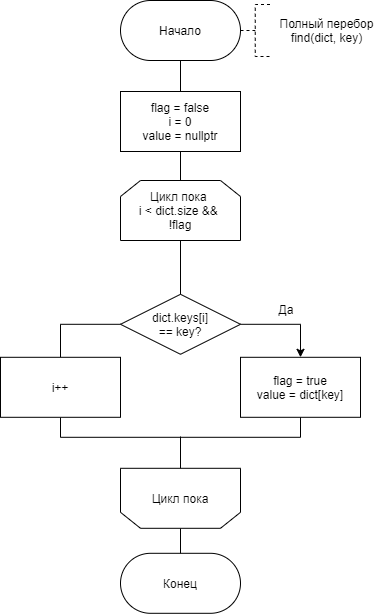
\includegraphics[scale = 0.65]{images/plunc_search.png}
	\caption{Полный перебор}
	\label{fig:plunc}
\end{figure}
\restoregeometry

Схема алгоритма бинарным поиском представлена на рисунке \ref{fig:binary}.
\begin{figure}[H]
	\centering
	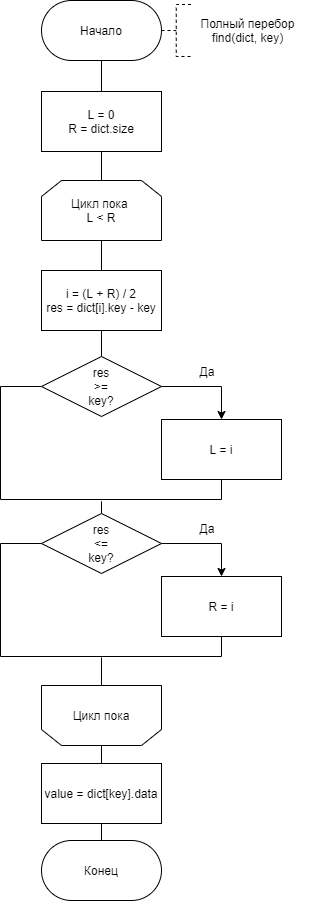
\includegraphics[scale = 0.55]{images/bin_search.png}
	\caption{Бинарный поиск}
	\label{fig:binary}
\end{figure}

Схема алгоритма поиска в словаре при его сегментировании представлена на рисунке \ref{fig:segment}.
\begin{figure}[H]
	\centering
	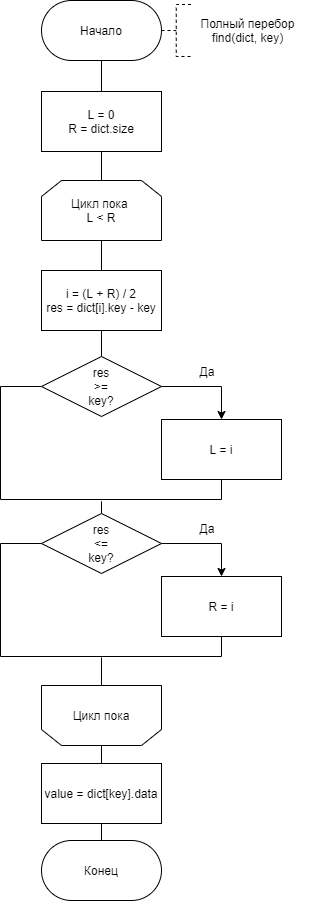
\includegraphics[scale = 0.53]{images/bin_search.png}
	\caption{Поиск в сегментах}
	\label{fig:segment}
\end{figure}

\section{Структура ПО}
В качестве аргумента командной строки программе передаётся файл, в котором содержится информация для словаря, и строки, являющиеся ключами, по которым осуществляется поиск.

\section{Классы эквивалентности}
Для осуществления функционального тестирования ПО были выделены следующие классы эквивалентности:
\begin{itemize}
	\item поиск первого ключа;
	\item поиск последнего ключа;
	\item поиск несуществующего ключа;
	\item поиск четного ключа;
	\item поиск нечетного ключа.
\end{itemize}

\section{Выводы}
На основе теоретических данных, приведенных в аналитическом разделе, были составлены схемы алгоритмов для их дальнейшей реализации в технологической части.
\newpage
\chapter{Технологическая часть}
Данный раздел содержит обоснование выбора языка и среды разработки, реализацию алгоритмов.

\section{Средства реализации}
Для реализации программы был выбран язык программирования Python~\cite{python}. Такой выбор обусловлен следующими причинами:
\begin{itemize}
	\item имеется большой опыт разработки;
	\item имеет большое количество расширений и библиотек, в том числе библиотеку для работы с потоками, измерения времени, построения графиков;
	\item обладает информативной документацией;
\end{itemize}

\section{Реализация алгоритмов}
В листингах \ref{lst:conv1} - \ref{lst:conv2} представлены реализации рассматриваемых алгоритмов.
%\newpage
\captionsetup{singlelinecheck=false, justification=raggedright}
\begin{lstlisting}[label={lst:conv1},caption=Реализация алгоритма поиска полным перебором]
def search_simple(key, animals_dict):
	cnt = 0
	for dict_key in animals_dict.keys():
		cnt += 1
		if key == dict_key:
		return animals_dict[key], cnt
	return None, 0
\end{lstlisting}
\newpage
\begin{lstlisting}[caption=Реализация алгоритма бинарного поиска]
def bin_search(key, animal_dict):
	keys = list(animal_dict.keys())
	cnt = 0
	i = 0
	j = len(animal_dict) - 1
	m = int(j / 2)

	while keys[m] != key and i < j:
		cnt += 1
		if key > keys[m]:
			i = m + 1
		else:
			j = m - 1
		m = int((i + j) / 2)
	cnt += 1
	if keys[m] != key:
		return None, cnt
	else:
		return animal_dict[keys[m]], cnt
\end{lstlisting}
\begin{lstlisting}[label={lst:conv2},caption=Реализация алгоритма поиска по сегментам]
def combined_search(key, seg_dict):
	cur_dict = {}
	a = key[0]
	cnt = 0
	if a < 'A' or a > 'Z':
		return None, 0
	else:
		for i in seg_dict.keys():
			cnt += 1
			if i == key[0]:
				cur_dict = seg_dict[i]
				break
		if len(cur_dict) == 0:
			return None, 0
		r, c = bin_search(key, cur_dict)
		return r, c+cnt
\end{lstlisting}

\section{Трудоемкость}
Так как функцией, оказывающей основную нагрузку на алгоритм является сравнение строк-ключей, теоретическая трудоемкость определяется как необходимое количество сравнений.\par
\subsection{Трудоемкость полного перебора}
Лучший случай для алгоритма поиска полным перебором наступает, если искомый ключ находится в первом элементе массива. В этом случае количество сравнений ключей определяется, как $f_{best} = 1$. В худшем случае, если ключ находится в последнем элементе массива или не содержится в нем, количество сравнений равняется $f_{worst} = N = 3350$. Медианная трудоемкость определяется, как $f_{median} = \frac{\sum_{i = 1}^{N} (i) + N}{N} \approx \frac{1 + N}{2N} \cdot N + N \approx \frac{N}{2} = 1675$\par
\subsection{Трудоемкость бинарного поиска}
Лучший случай для алгоритма бинарного поиска наступает, если искомый ключ находится точно в середине массива. В этом случае количество сравнений ключей определяется, как $f_{best} = 1$. В худшем случае, если ключ, например, отсутствует в массиве, количество сравнений равняется $f_{worst} = \log N + 1 = 13$. Медианная трудоемкость определяется, как $f_{median} = \frac{\sum_{i = 1}^{\log N} (i \cdot 2^{i + 1})}{N} =  \frac{2^{\log N} \cdot \log N - 2^{\log N} + 1}{N} \approx \frac{N \cdot \log N - N}{N} \approx \log N = 12$\par
\subsection{Трудоемкость поиска в словаре, разбитом на сегменты}
Поиск в словаре, разбитом на сегменты, аналогично поиску полным перебором требует $f_{best} =2$ сравнений в лучшем случае (элемент находится в первом сегменте в начале). Худший случай наступает для последнего сегмента, состоящего из наименьшего количества значений (5) и равняется, соответственно, $f_{worst} = \log 5 + 26 = 28$. Для сформированного словаря медианный случай требует в среднем $f_{median} = 14.4$ сравнений 

\section{Тестирование}
Тестирование реализованных алгоритмов проходило по методу "черного ящика". В таблице \ref{table::testing} описаны проверяемые тестовые случаи. Столбцу "вид" соответствует название биологического вида, столбцу "Научное название" - соответствующая информация. Фактические результаты тестов совпали с ожидаемыми.

\begin{table} [!h]
	\begin{center}
		
		\captionsetup{justification=raggedleft}
		\caption{Таблица тестовых данных}
		\label{table::testing}
		
		\begin{tabular}{| c || c |} 
			\hline
			Вид & Научное название\\
			\hline \hline
			Aardwolf&Proteles cristatus\\
			Zungaropsis multimaculatus & Zwackhiomyces dispersus \\
					&(J. Lahm ex Körb.) Triebel \& Grube\\
			aedfgh & Ключ не найден\\
			Ginseng & Panax pseudoginseng Wall.\\
			Florida Sphagnum & Sphagnum macrophyllum Brid. \\
					&var. floridanum Austin\\
			\hline
		\end{tabular}
	\end{center}
\end{table}

\section{Выводы технологической части}
В данном разделе были реализованы и протестированы алгоритмы поиска в словаре по ключу.

\section*{Вывод}
В этом разделе обоснован выбор языка програмирования, описаны технические характеристики,приведены листинги кода и оценка трудоемкости реализованных алгоритмов, проведены тесты.
\newpage

\chapter{Экспериментальная часть}
В данном разделе сравниваются реализованные алгоритмы, дается сравнительная оценка затрат на время.

\section{Пример работы программы}
Пример работы программы представлен на рисунке \ref{fig:ex}. 
\captionsetup{singlelinecheck=true}
\begin{figure}[H]
	\centering
	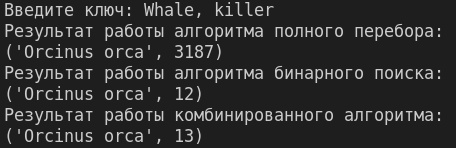
\includegraphics[width=1\linewidth]{images/ex}
	\caption{Пример работы программы}
	\label{fig:ex}
\end{figure}

\section{Технические характеристики}
Технические характеристики устройства, на котором выполнялось исследование:
\begin{itemize}
	\item операционная система: Ubuntu 20.01 Linux x86\_64~\cite{ubuntu};
	\item оперативная память: 8 Гб;
	\item процессор: AMD Ryzen5 4500U~\cite{processor}:
	\begin{itemize}
		\item количество физических ядер: 6;
		\item количество логических ядер: 6.
	\end{itemize}
\end{itemize}
В данном разделе проводится сравнительный анализ реализованных алгоритмов по затратам процессорного времени.

\section{Сравнительный анализ алгоритмов по количеству сравнений}
Гистограмма, визуализирующая необходимое количество сравнений для нахождения заданного ключа полным перебором представлена ниже, на рисунке \ref{fig:plunc_keys}.

Аналогичные рисунки представлены для алгоритма бинарного поиска (\ref{fig:bin_keys}), а также для поиска в сегментированном словаре (\ref{fig:seg_keys}).

На рисункax \ref{fig:bin_comp}  и \ref{fig:seg_comp} изображено, какие ключи будут найдены в массиве ключей за указанное число сравнений для алгоритмов бинарного поиска и поиска в сегментированном словаре соответственно, для алгоритма полного перебора такая гистограмма совпадает с гистограммой, описанной выше.

На представленных диаграммах видно, что количество сравнений при поиске полным перебором прямо пропорционально нормеру, под которым ключ находится в массиве.
Количество сравнений при бинарном поиске не имеет какой-либо выраженной 
зависимости от номера ключа. 
Для сегментированного словаря количество сравнений зависит от принадлежности конкретному сегменту, поэтому общее количество сравнений выше, чем для алгоритма бинарного поиска, что обуславливается довольно малым размером исходного словаря (3349 ключей) и неравномерным распределением значений в сегментах.

\captionsetup{justification=centerlast, singlelinecheck=false}
\begin{figure}[H]
	\centering
	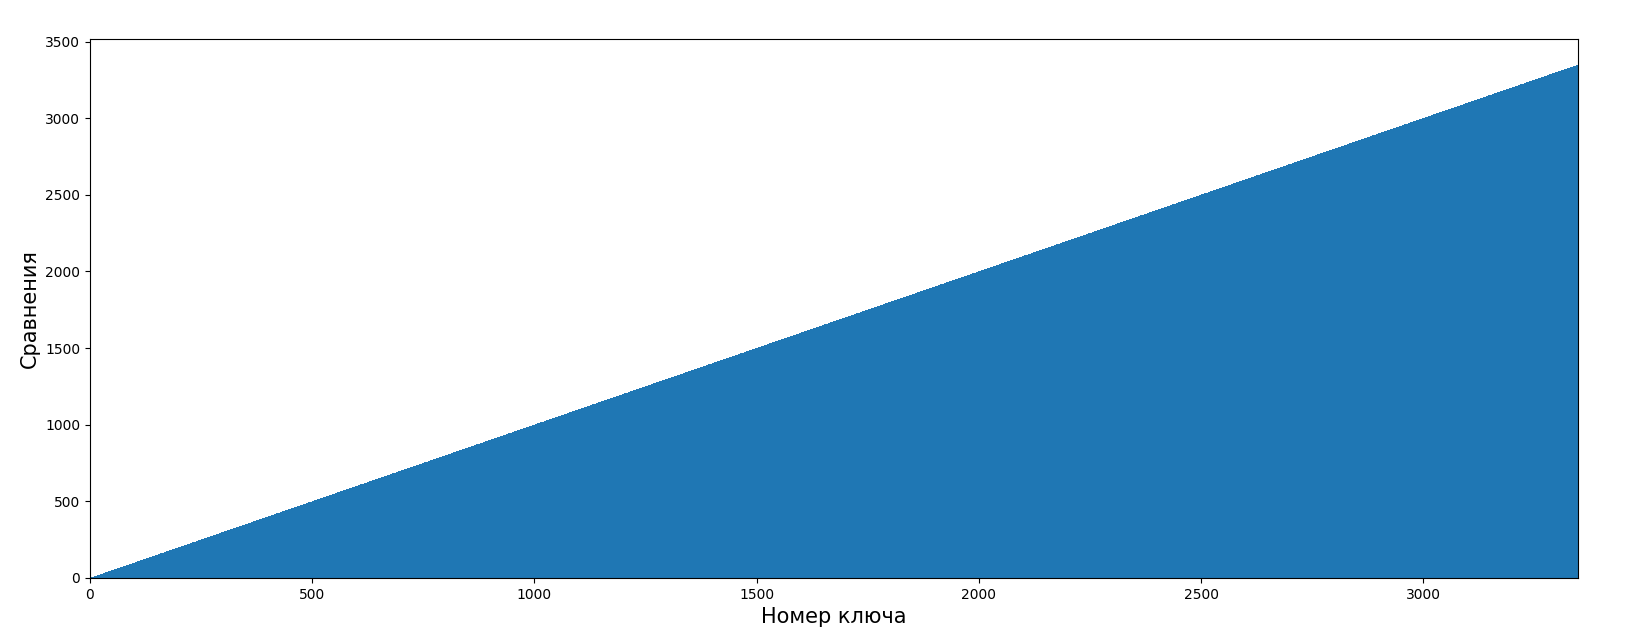
\includegraphics[scale = 0.3]{images/plunc_keys.png}
	\caption{Полный перебор}
	\label{fig:plunc_keys}
\end{figure}

\begin{figure}[H]
	\centering
	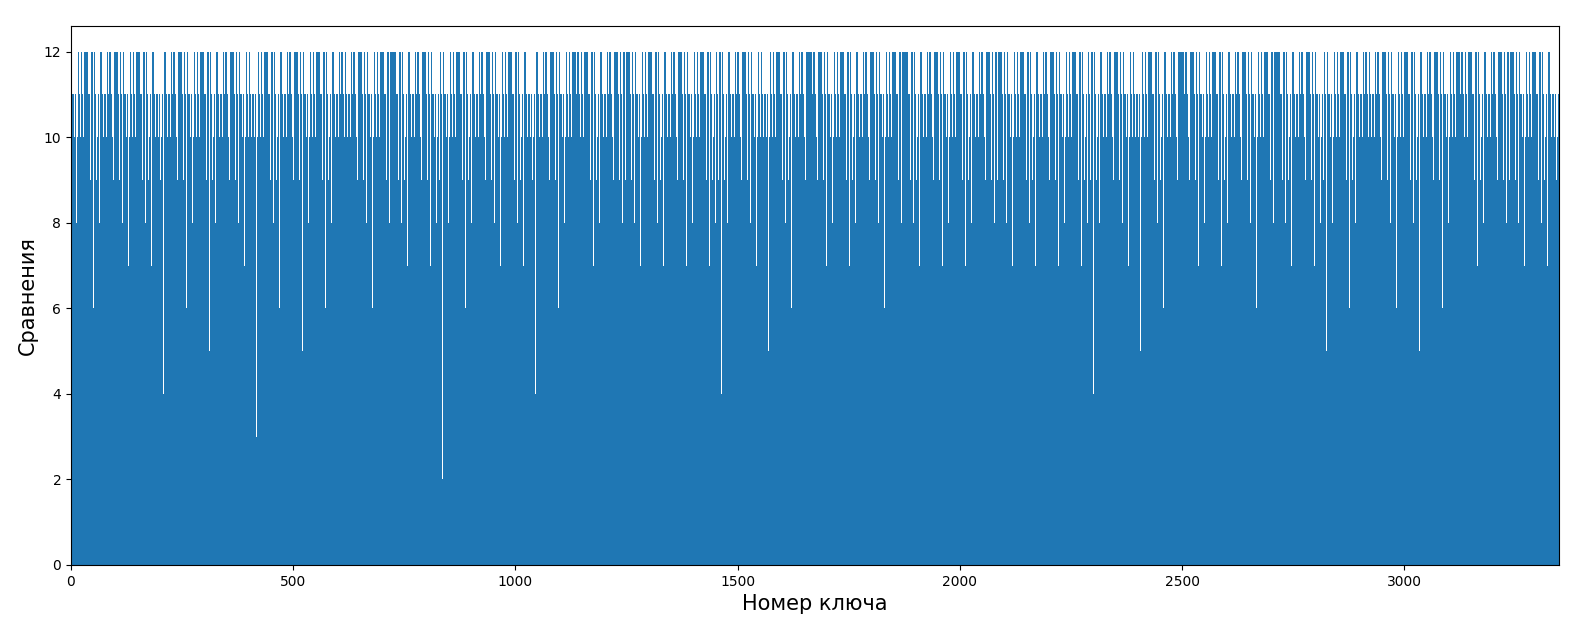
\includegraphics[scale = 0.3]{images/bin_keys.png}
	\caption{Бинарный поиск (часть 1)}
	\label{fig:bin_keys}
\end{figure}

\begin{figure}[H]
	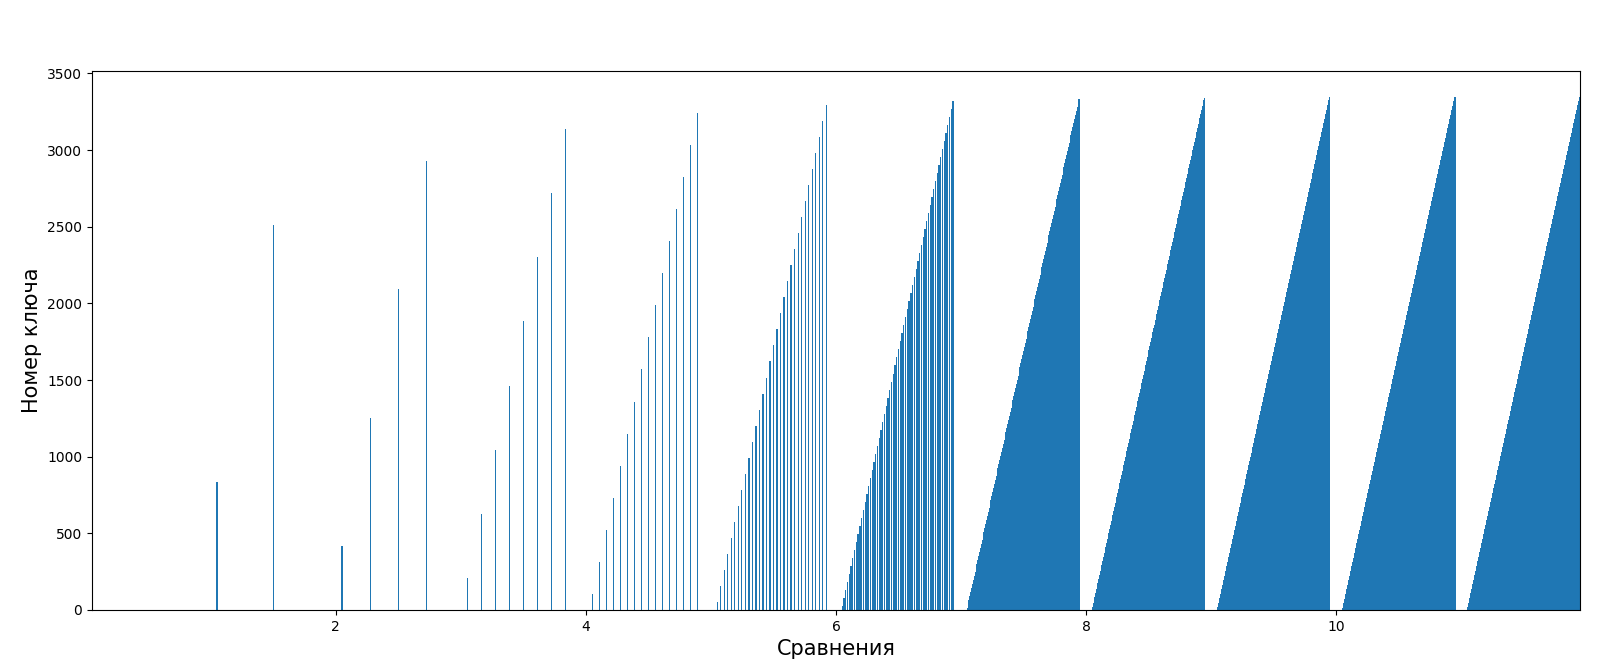
\includegraphics[scale = 0.3]{images/bin_comp.png}
	\centering
	\caption{Бинарный поиск (часть 2)}
	\label{fig:bin_comp}
\end{figure}

\begin{figure}[H]
	\centering
	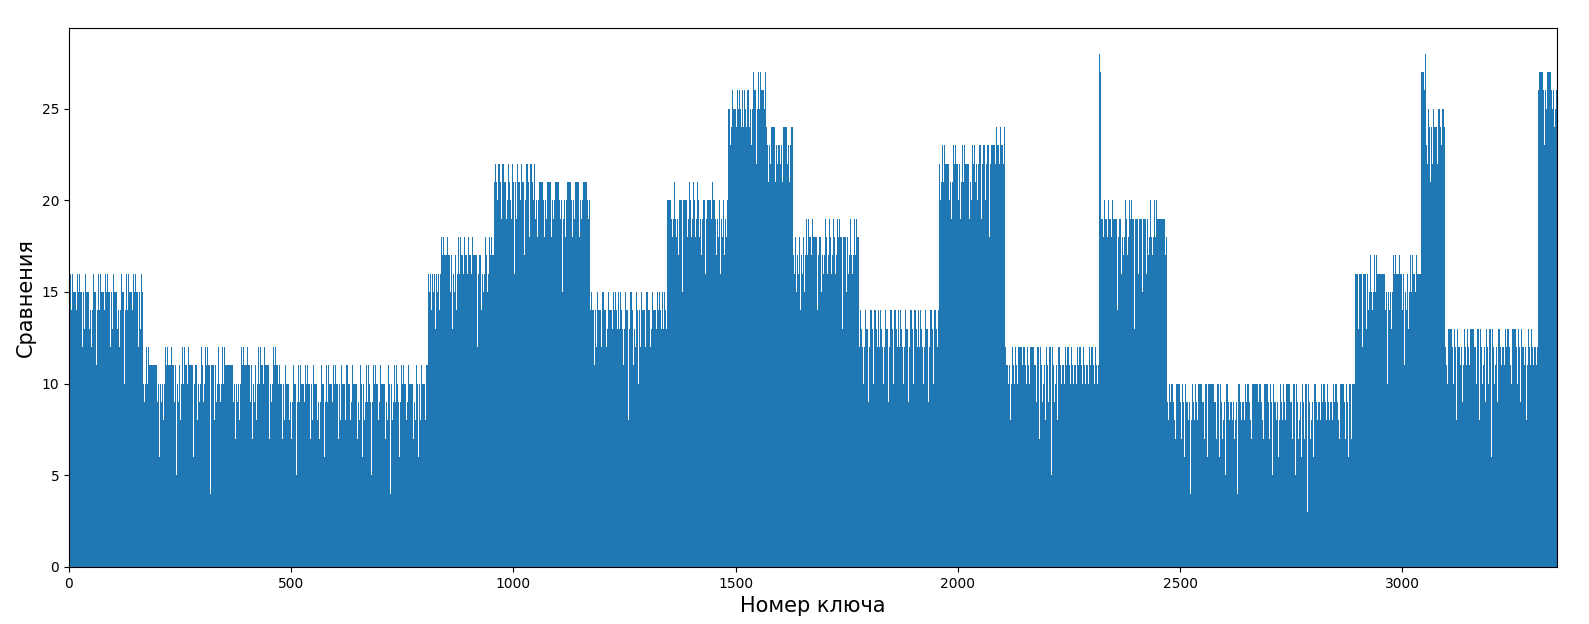
\includegraphics[scale = 0.3]{images/seg_keys.png}
	\caption{Сегментированный словарь (часть 1)}
	\label{fig:seg_keys}
\end{figure}

\begin{figure}[H]
	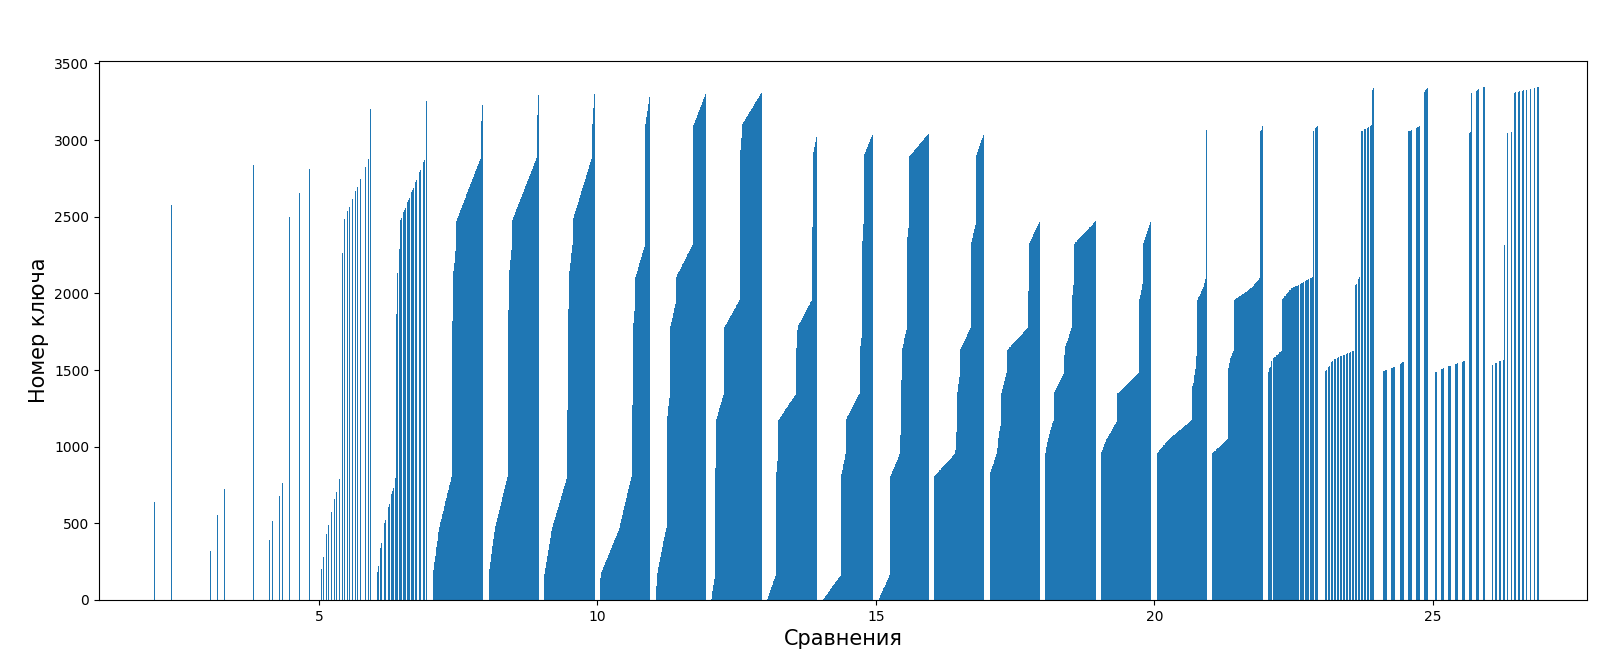
\includegraphics[scale = 0.3]{images/seg_comp.png}
	\centering
	\caption{Сегментированный словарь (часть 2)}
	\label{fig:seg_comp}
\end{figure}

\section{Выводы}
Бинарный алгоритм требует в среднем меньше сравнений, чем алгоритм полным перебором. Максимальное количество сравнений при поиске в сегментированном словаре больше аналогичного показателя при бинарном поиске. При одинаковом количестве сравнений, поиск в сегментированном словаре найдет ключ чаще, чем при бинарном поиске. Поиск в сегментированном словаре тем эффективней, чем равномерней распределeны значения исходного массива по сегментам.
\newpage

\addcontentsline{toc}{chapter}{Заключение}
\chapter*{Заключение}
В процессе выполнения работы изучены алгоритмы поиска в словаре.\\

Все поставленные задачи выполнены.
\begin{enumerate}
	\item Изучены способы поиска по ключу в словаре.
	\item Реализованы и протестированы алгоритмы поиска полным перебором, бинарным поиском и бинарным поиском в сегментированном словаре.
	\item Определена теоретическая трудоемкость алгоритмов, выраженная в количестве необходимый сравнений.
	\item Экспериментально установлено уменьшение максимального необходимого числа сравнений и среднего необходимого числа сравнений при бинарном поиске в случае, если словарь является сегментированным.
	\item Определены шаблоны распределения ключей от количества проведенных сравнений при бинарном поиске по массиву ключей.
\end{enumerate}
\newpage
\addcontentsline{toc}{chapter}{Список литературы}

\bibliographystyle{utf8gost705u}
\bibliography{bib_lab_7}
\nocite{*}
\end{document}